\documentclass[12pt,t]{beamer}
\usetheme[style=simple,nat,en]{Frederiksberg}
\usepackage{pslatex}
\usepackage{xmpmulti}
\usepackage[utf8]{inputenc}
\usepackage{color}
\usepackage{graphicx}
\usepackage{tikz}
\usepackage{listings}
\usepackage{xcolor}
\usetikzlibrary{arrows,automata,fit}
\usepackage{listings}% http://ctan.org/pkg/listings
\usepackage{animate}
\lstset{
      basicstyle=\ttfamily,
        mathescape
    }
% \setbeamercovered{transparent}

\definecolor{bluekeywords}{rgb}{0,0,1}
\definecolor{greencomments}{rgb}{0,0.5,0}
\definecolor{redstrings}{rgb}{0.64,0.08,0.08}
\definecolor{xmlcomments}{rgb}{0.5,0.5,0.5}
\definecolor{types}{rgb}{0.17,0.57,0.68}

\lstset{language=[Sharp]C,
captionpos=b,
%numbers=left, %Nummerierung
%numberstyle=\tiny, % kleine Zeilennummern
frame=lines, % Oberhalb und unterhalb des Listings ist eine Linie
showspaces=false,
showtabs=false,
breaklines=true,
showstringspaces=false,
breakatwhitespace=true,
escapeinside={(*@}{@*)},
commentstyle=\color{greencomments},
morekeywords={partial, var, value, get, set},
keywordstyle=\color{bluekeywords},
stringstyle=\color{redstrings},
basicstyle=\ttfamily\small,
}


\title{Cache optimizations in \\ Garbage Collection}
\subtitle{Bachelor Thesis}
\author{David Himmelstrup}
\institute{Department of Computer Science}

\begin{document}

\frame[plain]{\titlepage}
%% Første rigtige slide
\begin{frame}
    \frametitle{Overview}
    \begin{enumerate}
        \item Objectives
        \item Design
        \item Implementation
        \item Testing
        \item Possible improvements
    \end{enumerate}
\end{frame}

\begin{frame}
    \frametitle{Memory management}
    Top 10 programming languages (GitHub 2017):
    \begin{enumerate}
        \item {\color<2->{blue} Javascript}
        \item {\color<2->{blue} Python}
        \item {\color<2->{blue} Java}
        \item {\color<2->{blue} Ruby}
        \item {\color<2->{blue} PHP}
        \item {\color<2->{lightgray} C++}
        \item {\color<2->{blue} C\#}
        \item {\color<2->{blue} Go}
        \item {\color<2->{lightgray} C}
        \item {\color<2->{blue} Swift}
    \end{enumerate}
\end{frame}


%\begin{frame}
    \frametitle{State Machine Design}
    \begin{figure}
      \begin{center}
        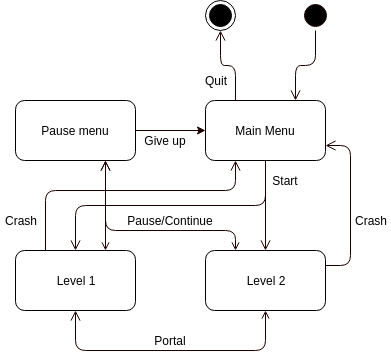
\includegraphics[height=0.7\textheight]{StateMachine.png}
      \end{center}
    \end{figure}
\end{frame}

%\begin{frame}
    \frametitle{Physics}
    \begin{itemize}
        \item Gravity equation: $ v(t_1) \approx a(t_0) \times \Delta t + v(t_0)$
        \item Gravity as a strategy / SOLID
        \item Playability: Ceiling on speed from gravity
        \item Thrusters can apply force left, right and up but not down
        \item Forces are defined as screen sizes per tick
        \item Thrust force is 0.01\% screen height/width per tick${}^2$
        \item Gravity is 0.005\% screen height per tick${}^2$
    \end{itemize}
\end{frame}

%\begin{frame}
    \frametitle{Collision Detection}
    \begin{itemize}
        \item StateMachine responsible for acting on collisions
        \item High level API in Level class (checks for collisions with walls and platforms)
        \item StateMachine responsible for collision logic
        \item StateMachine responsible for making platforms solid
    \end{itemize}
\end{frame}

%\begin{frame}
    \frametitle{Scoring points}
    \begin{itemize}
        \item Customers spawn after the player enters a level with a delay
        \item Score class can render itself
        \item StateMachine updates the score state
        \item Room for just 1 customer per trip
    \end{itemize}
\end{frame}

%\begin{frame}
    \frametitle{Level classes layout}
    \begin{figure}
      \begin{center}
        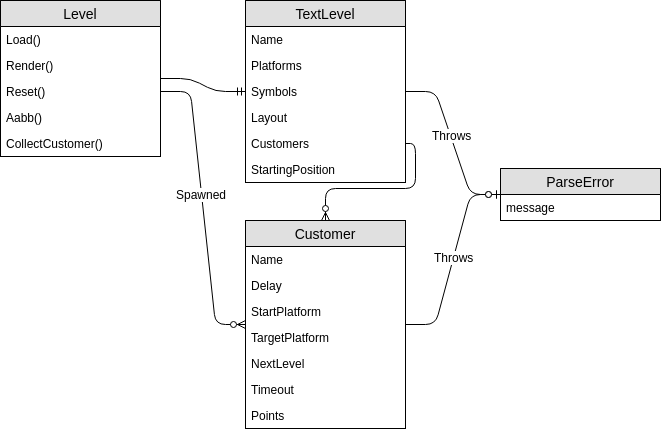
\includegraphics[height=0.7\textheight]{LevelUML.png}
      \end{center}
    \end{figure}
\end{frame}

%\begin{frame}
    \frametitle{Use case analysis}
    \begin{figure}
      \begin{center}
        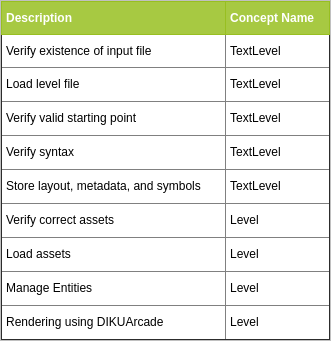
\includegraphics[height=0.7\textheight]{UseCase.png}
      \end{center}
    \end{figure}
\end{frame}


%\begin{frame}
    \frametitle{Parser implementation}
    \pause
    \begin{itemize}
        \item No parser library
        \pause
        \item Repeated sanity checks
        \pause
        \item Edge-cases and maintainability
    \end{itemize}
\end{frame}

%\begin{frame}[fragile]
    \frametitle{Parser implementation}

\begin{lstlisting}
Name = Prefixed("Name: ", ExpectLine(lines));

string platformsLine = Prefixed("Platforms: ", ExpectLine(lines));
Platforms = platformsLine.Split(
              new[] {", "},
              StringSplitOptions.None);
\end{lstlisting}
\end{frame}


%\begin{frame}
    \frametitle{Testing}
    \begin{enumerate}
        \item White box, unit testing
        \begin{itemize}
          \item Correctness check for level 1 and 2
          \item Error handling checks
          \item Full coverage checks for customer parsing
        \end{itemize}
        \item Black box, integration testing
        \begin{itemize}
          \item Compile and run game
          \item Navigate entire state machine
          \item Collect and deliver customers
          \item Crash into walls
        \end{itemize}
    \end{enumerate}
\end{frame}

%\begin{frame}
    \frametitle{Improvements}
    \begin{itemize}
        \item Parsing (Parseq, Parsley, Pidgin)
        \item Bitmap Collision detection
        \item State machine tests
        \item Customer animations
        \item Additional maps
    \end{itemize}
\end{frame}

%\begin{frame}
    \frametitle{Gameplay}
    \begin{figure}
      \begin{center}
        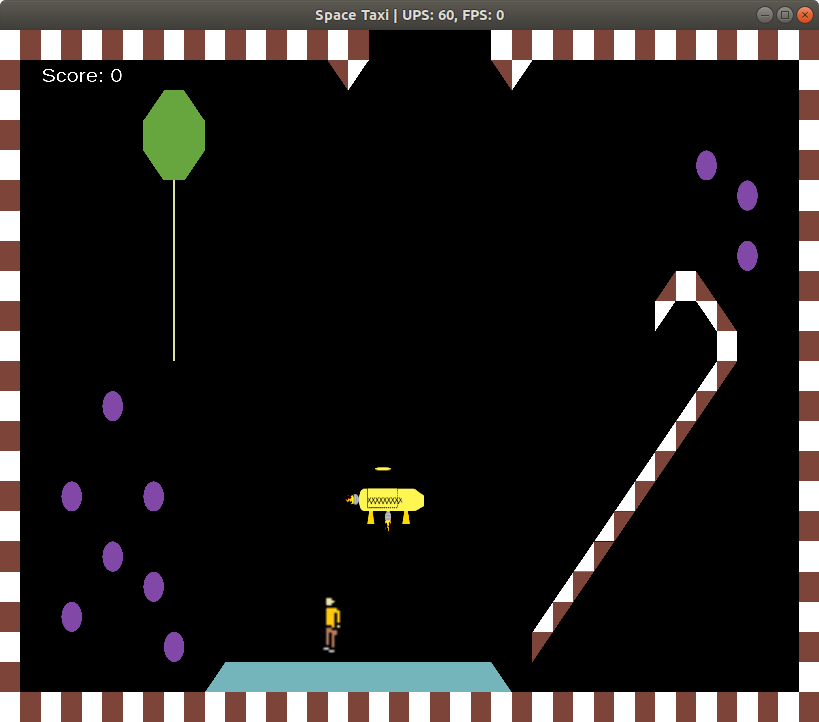
\includegraphics[height=0.7\textheight]{GamePlay.png}
      \end{center}
    \end{figure}
\end{frame}


\end{document}
